\documentclass{../cpct/ctpro}

\title{ACM 算法实验室 22 届成员选拔赛}
\date{2022 年 10 月 16 日}

\begin{document}

\maketitle
\addproblem{Zxilly 的饼}{1000}{256}{传统}{Algor}
\addproblem{置换反应}{1000}{256}{传统}{AgOH}
\addproblem{集和}{1000}{256}{传统}{AgOH}
\addproblem{购物}{1000}{256}{传统}{GlenBzc}
\addproblem{队形摆好}{1000}{256}{传统}{Zxilly}
\addproblem{最近等值对}{2000}{256}{传统}{Algor}
\addproblem{井字棋}{1000}{256}{传统}{Algor}
\addproblem{表演型卷王}{1000}{256}{传统}{Tifa}
\addproblem{跃迁}{1000}{256}{传统}{AgOH}


\section*{比赛信息}

\begin{remark}
    \textbf{A $\sim$ F 题为萌新组题目,D $\sim$ I 题为老鸟组题目。}
\end{remark}

\ctinfotab{IOI}{C/C++,~Python,~Java}{3}

\section*{题目概况}

\problemtab

\section*{编译命令}

参见 OJ 帮助

\section*{注意事项}

\begin{itemize}
    \item C/C++ 中函数 \lstinline{main()} 的返回值类型必须是 \lstinline{int},程序正常结束时的返回值必须是 $0$。
    \item C/C++ 代码必须完全符合 GNU C/C++ 标准,不能使用诸如绘图、Win32API、中断调用、硬件操作或与操作系统相关的API。
    \item C/C++ 代码中允许使用 STL 类库。
\end{itemize}

\paragraph*{} 祝大家取得好成绩!

\makeproblem
\section*{题目描述}

Zxilly 手中有一张总量为 $m$ 的饼,由于 Zxilly 太饿了,需要在 $n$ 口内吃完这张饼。

Zxilly 想在吃饼的同时考一考你的数学,所以他告诉了你第 $i$ 口能吃掉的量 $a_i$,请你告诉 Zxilly 他能不能在 $n$ 口内吃完这张饼。如果能,回答 \texttt{YES} 并告诉他在第几口吃完;如果不能,回答 \texttt{NO} 并告诉他饼还剩多少。

\section*{输入格式}

第一行,两个整数 $m,n$。

第二行,$n$ 个整数 $a_i$。

\section*{输出格式}

一行,若能吃完,输出 \texttt{YES} 和第几口吃完;若不能吃完,输出 \texttt{NO} 和饼的剩余量。

\section*{输入输出样例}

\testcasetab
{
    5 3 \par
    1 2 3
}
{
    YES 3
}

\testcasetab
{
    8 3 \par
    1 2 3
}
{
    NO 2
}

\section*{说明/提示}

对于 $50 \%$ 的测试数据,$1 \leq m \leq 1 \times {10}^9$。

对于所有的测试数据,$1 \leq m \leq 1 \times {10}^{18},~1 \leq n \leq 1 \times {10}^6,~1 \leq a_i \leq 1 \times {10}^9$。

\makeproblem
\section*{题目描述}

置换反应是单质与化合物反应生成另外的单质和化合物的化学反应,其化学反应方程式形如以下格式:

$$A+BC \longrightarrow AC+B$$

简单起见,设其中 $A,B,C$ 都是元素。元素是一个由大写字母开头且最多包含一个大写字母的,长度为 $1$ 或 $2$ 的字符串,例如 \texttt{C} 和 \texttt{Zn} 都是元素,但 \texttt{og}、\texttt{Cmd}、\texttt{ZZ} 不是元素。注意,可能存在并不在元素周期表内的元素,例如 \texttt{A} 或 \texttt{Cc}。

现给定一个置换反应的化学反应方程式的两个反应物,请你计算出反应的两个产物。

注意:本题存在多组数据。

\section*{输入格式}

第一行,一个整数 $t$,代表数据组数。

接下来 $t$ 行,每行两个字符串,分别代表 $A$ 与 $BC$。

\section*{输出格式}

$t$ 行,每行两个字符串,分别代表 $AC$ 与 $B$。

\section*{输入输出样例}
\testcasetab
{
    3 \par
    A BC \par
    K NaCl \par
    Ag ZnS
}
{
    AC B \par
    KCl Na \par
    AgS Zn
}

\section*{说明/提示}

\textbf{在 \lstinline{cctype} 头文件中}有两个可以判断一个字符是否小写/大写的函数:\lstinline{islower(char c)} 与 \lstinline{isupper(char c)},返回值为 \lstinline{bool} 类型,代表参数中给定的字符是否为小写/大写。

例如:\lstinline{islower('a')} 结果为 \lstinline{true};\lstinline{isupper('z')} 结果为 \lstinline{false};\lstinline{isupper('C')} 结果为 \lstinline{true}。

【数据规模】

对于 $100 \%$ 的数据,$1 \leq t \leq {10}^5$。

\makeproblem
\section*{题目描述}

对于任意有限数集 $A,B$,定义二者之和 $A+B$ 为:

$$A+B = \{x+y | x \in A,~y \in B \}$$

例如,当 $A=\{1,2 \},~B=\{3,4 \}$,有 $A+B = \{4,5,6 \}$。注意此处并非可重集,因此即使 $1+4 = 2+3 =5$,$A+B$ 也仅包含一个 $5$。

记有限数集 $A$ 中的元素个数为 $|A|$。

给定 $n$,设 $A=\{1,2,3,\cdots,n-1,n \}$,求 $|A+A|$。

注意:本题存在多组数据。

\section*{输入格式}

第一行,一个整数 $t$,代表数据组数。

接下来 $t$ 行,每行一个整数 $n$,意义见题目描述。

\section*{输出格式}

$t$ 行,每行一个整数,代表对应结果。

\section*{输入输出样例}
\testcasetab
{
    2 \par
    1 \par
    6
}
{
    1 \par
    11
}

\section*{说明/提示}

【样例解释】

对于第一个样例:$A = \{1 \},A+A = \{1+1 \} = \{2 \}$,故 $|A+A| = 1$。

【数据规模】

对于 $10 \%$ 的数据,$1 \leq n \leq 1000$。

对于 $30 \%$ 的数据,$1 \leq n \leq {10}^9$。

对于 $100 \%$ 的数据,$1 \leq t \leq {10}^5,~1 \leq n \leq {10}^{18}$。

\makeproblem
\section*{题目描述}

为了迎接新生到来,某超市决定进行促销活动。促销活动将会持续 $m$ 天,第 $i$ 天的促销形式为买 $x_i$ 件\textbf{免单} $y_i$ 件,但是精明的老板只会将 $x_i$ 件里\textbf{最便宜的} $y_i$ 件送给你,剩下的 $x_i-y_i$ 件商品你仍需正常付款。

超市内共有 $n$ 类商品,商品的价格为 $a_1, a_2,\cdots, a_n$,为了防止你薅羊毛,老板还规定你每天每种商品限购一件。

请问每天你能\textbf{免费}获得的最大商品总价值是多少。

\section*{输入格式}

第一行,两个整数 $n,m$ 表示商品总数和促销持续天数。

第二行,$n$ 个整数,表示每个商品的价格 $a_i$。

接下来 $m$ 行,每行两个整数 $x_i,y_i$ 表示买 $x_i$ 件商品免单 $y_i$ 件。

\section*{输出格式}

一行,一个整数,表示你能免费获得的最大商品总价值。

\section*{输入输出样例}
\testcasetab
{
    6 4 \par
    6 4 2 5 1 4 \par
    4 2 \par
    5 3 \par
    6 4 \par
    3 2
}
{
    8 \par
    10 \par
    11 \par
    9
}

\section*{说明/提示}

对于 $50 \%$ 的测试数据,$1 \leq n,m \leq 1000,~1 \leq x \leq y \leq 1000$。

对于 $100 \%$ 的测试数据,$1 \leq n,m \leq {10}^{6},~1 \leq x \leq y \leq {10}^{6},~1 \leq a_i \leq 2 \times {10}^5$。

【样例解释】

第一天选择购买 $x_1,x_2,x_4,x_6$,价格为 $a_1=6,a_2=4,a_4=5,a_6=4$,其中价格最便宜的两件 $x_2,x_6$ 获得免单,第一天免费获得的最大商品总价值为 $a_2+a_6=8$。

第二天选择购买 $x_1,x_2,x_3,x_4,x_6$,价格为 $a_1=6,a_2=4,a_3=2,a_4=5,a_6=4$,其中价格最便宜的三件 $x_2,x_6,x_3$ 获得免单,第二天免费获得的最大商品总价值为 $a_2+a_6+a_3=10$。

\makeproblem
\section*{题目描述}

某大学开学了,新生在操场上进行开学典礼。新生有 $n$ 个班,每个班有 $a_1,a_2,\cdots,a_n$ 人。班级在操场上从左至右纵向排列。

现在,校领导要求所有班级的长度都相同,即每个班级的队列人数都相同。为了实现这一目标,每个学生可以从一个班级的队伍的末尾走到另外一个班级的队伍的末尾,每个学生消耗的体力为两个班之间的距离 $k$。

校领导希望知道,最少共需要多少学生们的体力才能使所有班级的队伍长度相同。

\section*{输入格式}

第一行,一个整数 $n$,表示班级的数量。

第二行,$n$ 个整数 $a_1,a_2,\cdots,a_n$,表示每个班级的人数(当前队伍长度)。

\section*{输出格式}

一个整数,表示最少共需要多少体力。如果不可能使所有班级的队伍长度相同,则输出 $-1$。

\section*{输入输出样例}
\testcasetab
{
    5 \par
    20 40 60 80 100
}
{
    120
}

\testcasetab
{
    3 \par
    1 2 4
}
{
    -1
}

\section*{说明/提示}

【样例解释 \#1】

班级 $a_1,a_2,a_3,a_4,a_5$ 的人数分别为 $20,40,60,80,100$,总人数为 $300$,所以每个班级的人数应该为 $60$。

班级 $a_4$ 的 $20$ 个人走到班级 $a_2$,消耗的体力为 $20 \times |4-2| = 40$。

班级 $a_5$ 的 $40$ 个人走到班级 $a_1$,消耗的体力为 $40 \times |5-1| = 160$。

因此,总体力消耗为 $40+160=200$。

【样例解释 \#2】

班级 $a_1,a_2,a_3$ 的人数分别为 $1,2,4$,总人数为 $7$,所以每个班级的队伍长度不可能相同,输出 $-1$。

【数据范围】

对于 $20 \%$ 的数据,$~0 \leq a_i \leq 10$;

对于 $40 \%$ 的数据,$1 \leq n \leq 10$;

对于 $100 \%$ 的数据,$1 \leq n \leq {10}^5,~0 \leq a_i \leq {10}^9$。

\makeproblem
\section*{题目描述}

对于 $n$ 个整数 $a_1,a_2,a_3,\cdots,a_n$,请你找到一对整数 $p,q~(1 \leq p < q \leq n)$ 满足以下三个条件:

\begin{enumerate}
    \item $a_p = a_q$;
    \item 在条件 $1$ 的前提下 $q-p$ 最小;
    \item 在条件 $2$ 的前提下 $q+p$ 最小。
\end{enumerate}

若这样的 $p,q$ 存在,则输出 $p+q$,否则输出 $-1$。

\section*{输入格式}

第一行,一个整数 $n$。

第二行,$n$ 个整数 $a_i$。

\section*{输出格式}

一行,若这样的 $p,q$ 存在,输出 $p+q$ 的值,否则输出 $-1$。

\section*{输入输出样例}
\testcasetab
{
    5 \par
    1 2 1 2 3
}
{
    4
}

\testcasetab
{
    5 \par
    1 2 3 4 5
}
{
    -1
}

\section*{说明/提示}

【样例解释 \#1】

$\{1,3 \},\{2,4 \}$ 满足条件 $1$ 和条件 $2$,而只有 $\{1,3 \}$ 满足条件 $3$ 因此答案为 $1 + 3 = 4$。

【样例解释 \#2】

不存在任何一对整数 $p,q$ 满足条件 $1$,因此答案为 $-1$。

【数据范围】

对于 $30 \%$ 的测试数据,$1 \leq n,a_i \leq 1 \times {10}^{3}$。

对于所有测试数据,$1 \leq n \leq 1 \times {10}^{5},~1 \leq a_i \leq 1 \times {10}^{9}$。

\makeproblem
\section*{题目描述}

Algor 和 AgOH 玩井字棋,由于 Algor 太菜了所以 AgOH 决定每次都让 Algor 先手,即 Algor 的棋子一定是 \texttt{X},AgOH 的棋子一定是 \texttt{O},未落子的格子用 \texttt{.} 表示。给定一个井字棋的局面,请你判断局面的情况,具体请参考【输出格式】。

\section*{输入格式}

第一行,一个整数 $t$ 表示有 $t$ 组测试数据。

每组测试数据包含三行字符串,每个字符串包含三个字符,每个字符只可能是 \texttt{X},\texttt{O},\texttt{.} 三种之一,表示该位置的落子情况。

\section*{输出格式}

共 $t$ 行,第 $i$ 行表示第 $i$ 组测试数据的状态。

每组测试数据仅为以下几种情况之一:

\begin{itemize}
    \item \texttt{illegal!} — 当前状态在正常游戏中无法达成;
    \item \texttt{Algor win!} — 当前状态下 Algor 获胜;
    \item \texttt{AgOH win!} — 当前状态下 AgOH 获胜;
    \item \texttt{Algor now!} — 当前状态下轮到 Algor 落子;
    \item \texttt{AgOH now!} — 当前状态下轮到 AgOH 落子;
    \item \texttt{draw!} — 当前状态为平局。
\end{itemize}

\section*{输入输出样例}
\testcasetab
{
    2 \par
    XXX \par
    O.O \par
    O.X \par
    XOX \par
    XO. \par
    .O.
}
{
    Algor win! \par
    AgOH win!
}

\section*{说明/提示}

井字棋是经典的儿童游戏,两个人在 $3 \times 3$ 的棋盘上轮流落子,如果某一次落子使得棋盘上出现三个相同的棋子连成一条线(横三个,竖三个或斜三个)则当前玩家获胜,游戏结束;如果某次落子没有分出胜负并且棋盘被占满则宣布平局,游戏结束;任何不可能出现在正常游戏的棋盘上的情况均视为为非法情况。

【样例解释】

第一个样例状态如图,先手方 Algor 获胜:

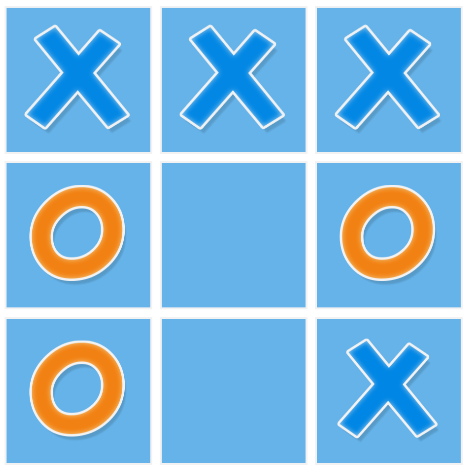
\includegraphics[scale=0.5]{images/1.png}

第二个样例状态如图,后手方 AgOH 获胜:


\includegraphics[scale=0.5]{images/2.png}

\makeproblem
\section*{题目描述}

开学了,Tifa 决定给自己营造一个新人设。因为 Tifa 觉得之前他学习不能说废寝忘食吧,也只能说是心猿意马了,所以 Tifa 决定这学期当一个卷王!

当然,Tifa 这种摆烂成性的人是不可能真的当卷王的,所以 Tifa 决定在宿舍有人的时候假装自己是卷王,没人的时候继续摆烂。根据 Tifa 对舍友的了解,每天只有在固定的一些时间段内才会有人在宿舍,Tifa 想知道自己还有多少时间能够摆烂。

因为 Tifa 不学无术,所以完全不会算,于是他向你求助。由于 Tifa 要急着打游戏,所以请在 1s 的时间内给出答案。

\section*{输入格式}

第一行为一个整数 $T$,表示数据组数。

每组数据的第一行为一个整数 $n$,表示时间段的个数,接下来 $n$ 行每行一个字符串,格式为 \texttt{hh:mm:ss-hh:mm:ss},表示在这段时间内有人在宿舍,保证所有时间段的开始时间严格小于结束时间。

\section*{输出格式}

对每组数据,输出一行字符串,格式为 \texttt{hh:mm:ss},表示 Tifa 可以休息的时长。

\section*{输入输出样例}
\testcasetab
{
    4 \par
    3 \par
    06:00:00-09:00:00 \par
    11:00:00-15:00:00 \par
    19:00:00-23:00:00 \par
    3 \par
    08:29:58-08:29:59 \par
    13:00:00-23:59:59 \par
    00:00:00-04:00:00 \par
    5 \par
    00:00:00-01:30:00 \par
    07:50:00-08:20:00 \par
    13:00:00-14:20:00 \par
    19:30:00-22:00:00 \par
    20:00:00-23:59:59 \par
    7 \par
    08:00:00-18:00:00 \par
    05:00:00-07:00:00 \par
    06:30:00-08:20:00 \par
    00:00:00-05:30:00 \par
    13:00:00-15:00:02 \par
    17:59:59-22:32:43 \par
    21:22:23-23:59:59
}
{
    12:59:57 \par
    08:59:57 \par
    16:09:57 \par
    00:00:00
}

\section*{说明/提示}

对于 $40 \%$ 的数据,$T = 1$;

对于 $60 \%$ 的数据(和上一种情况有重叠),$1 \leq n \leq 100$;

对于 $100 \%$ 的数据,$1 \leq T \leq 50,~1 \leq n \leq 1000,~0 \leq \texttt{hh} \leq 23,~0 \leq \texttt{mm},\texttt{ss} \leq 59$。

\makeproblem
\section*{题目描述}

原子周围由近到远分为 $n$ 个能级,分别叫做第 $1$ 能级、第 $2$ 能级、……、第 $n$ 能级。小 s 是一个活泼的电子,它生活在第 $1$ 能级,小 s 最好的朋友是一个叫做小 y 的电子,它生活在第 $n$ 能级。

某天,小 s 想要去找小 y 玩,因为小 s 是一个电子,所以小 s 只能通过一种叫做“跃迁”的方式移动。跃迁具有一定随机性,也就是说在某一时刻,小 s 将以相同的概率随机移动到它所在能级的上一个能级或下一个能级,并花费 $1$ 秒的时间。

注意:小 s 在第 $1$ 能级时,它只能花费 $1$ 秒的时间跃迁到第 $2$ 能级;因为小 s 非常活泼,所以小 s 每秒一定会发生跃迁,不会原地不动。

请问小 s 期望需要花费多少秒才能从第 $1$ 能级移动到第 $n$ 能级见到小 y 呢?

形式上说,共有 $n$ 个格子 $a_1,a_2,\cdots,a_n$,若当前在格子 $a_i~(i \neq 1)$ 上,则下一秒就可能在格子 $a_{i-1}$ 或 $a_{i+1}$ 上,问从 $a_1$ 移动到 $a_n$ 期望需要花费多少秒。

\section*{输入格式}

一行,一个整数 $n$。

\section*{输出格式}

若结果为一个整数,直接输出这个整数;若结果为一个分数,输出分子和分母,中间用空格隔开。

\section*{输入输出样例}
\testcasetab
{
    1
}
{
    0
}

\testcasetab
{
    2
}
{
    1
}

\testcasetab
{
    42
}
{
    65420941852673 549755813888
}

\section*{说明/提示}

对于 $40 \%$ 的数据,$1 \leq n \leq 20$。

对于 $100 \%$ 的数据,$1 \leq n \leq 50$。

\end{document}
